\chapter{Gewöhnliche Differenzialgleichungen}
Eine Gleichung, in der Ableitungen einer gesuchten Funktionen auftreten, nennt man Differentialgleichung.
\begin{align*}
y'(t)&=y+y^2\\
\left( y'(t)\right)^2&=y(t)+2
\end{align*}

Hängt die gesuchte Funktion in der DGL nur von einer einzigen Variablen ab, so spricht man von einer ``gewöhnlichen DGL''.\\

Hängt hingegen die gesuchte Funktion von mehrere Variabeln ab, d.h. kommen partielle Ableitungen in der Differentialgleichung vor, so liegt eine ``partielle DGL'' vor. Viele physikalische Prozesse lassen sich oft durch Differenzialgleichungen beschreiben.
\subsubsection*{Beispiel}
\begin{enumerate}
\item Ein lineares Federpendel wird durch folgende DGL beschrieben \[m\frac{d^2x}{dt^2}=-Kx \text{  mit K = Federkonstante}\]
\begin{center}
\begin{tikzpicture}
\node[circle,fill=black,inner sep=1.5mm] (a) at (0,0) {};
\draw[decoration={aspect=0.3, segment length=2mm, amplitude=2mm,coil},decorate] (2,0) -- (0.5,0);
\draw[decoration={aspect=0.3, segment length=2mm, amplitude=2mm,coil},decorate] (-2,0) -- (-0.5,0);
\draw (0.5,0)--(0,0);
\draw (-0.5,0)--(0,0);
\draw (2,0)--(2.5,0);
\draw (-2,0)--(-2.5,0);

\fill [pattern = north east lines] (-2.5,-0.5) rectangle (-2.7,0.5);
\draw[thick] (-2.5,0.5) -- (-2.5,-0.5);
\fill [pattern = north east lines] (2.5,-0.5) rectangle (2.7,0.5);
\draw[thick] (2.5,0.5) -- (2.5,-0.5);

\draw[] (0,-0.8) -- (0,-0.3);
\draw[->] (0,-0.55) -- (1,-0.55);
\node[] at (1.5,-0.55){$x(t)$};
\end{tikzpicture}
\end{center}
Unbekannt ist hier die Auslenkung $x$ in Abhängigkeit von der Zeit $t$
\item Beim radioaktiven Zerfall haben wir \[\frac{df(t)}{dt}=-\alpha f\text{\hspace{10mm}}f(0)=f_0\]
wobei $f(t)=$ die noch vorhandeden Masse eines Stoffes. Die pro Zeiteinheit zerfallende Masse ist proportional zur noch vorhandenen Masse.
\item Freier Fall mit Reibung
\begin{center}
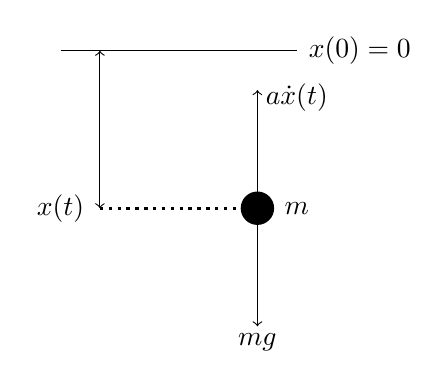
\begin{tikzpicture}
\node[circle,fill=black,inner sep=1.5mm] (a) at (0,0) {};
\draw[<->](-2,0)--(-2,2);
\draw[->] (0,0) -- (0,1.5);
\draw[->] (0,0) -- (0,-1.5);
\draw[] (-2.5,2) -- (0.5,2);
\draw[dotted, very thick] (-2,0) -- (0,0);
\node[] at (-2.5,0){$x(t)$};
\node[] at (1.3,2){$x(0)=0$};
\node[] at (0.5,0){$m$};
\node[] at (0.5,1.4){$a\dot x(t)$};
\node[] at (0,-1.7){$mg$};
\end{tikzpicture}
\end{center}
Sei $m$ ein Massepunkt der unter Einfluss der Schwerkraft fällt. Es kann auch eine Reibungskraft geben. \\

Die Grösse der Reibungskraft ist proportional zur Geschwindigkeit. Dann ist, nach dem zweiten Newtonschen Gesetz \[m\ddot x = mg - a\dot x\text{\hspace{10mm}}v=\frac{dx}{dt}\]
Beim Beispiel 2., haben wir schon letztes Semester gesehen dass \[\frac{df(t)}{dt}=-\alpha f\] als eine Lösung $Ke^{-\alpha t}$, $K\in\R$, hat
\begin{align*}
f'=-\alpha f\Rightarrow \frac{f'}{f}&=-\alpha\\
\int{\frac{f'(t)}{f(t)}dt}&=-\int{\alpha dt}\\
\ln\abs{ f(t)}&=-\alpha t+C\\
\Rightarrow f(t)&=Ke^{-\alpha t}\text{ mit }K={e^C}
\end{align*}

\end{enumerate}
Alle drei Beispiele sind lineare DGL mit konstanten Koeffizienten.
\section{Lineare DGL mit konstanten Koeffizienten}

\begin{definition}{7.1}
Eine lineare Differentialgleichung $n-$ter Ordnung hat die Gestalt \[{y^{(n)}} + {a_{n - 1}}(x){y^{(n - 1)}} +  \ldots  + {a_1}(x)y' + {a_0}(x)y = b(x)\] mit $a_i(x),i=0,\dots,n-1, b(x)$ Funktionen. \\

Ist die sogenannte Störfunktion $b(x)$ konstant gleich 0, so heisst die DGL homogen, andernfalls inhomogen. Im Falle $a_i(x)=a_i$ Konstanten, heisst die LDG, LDG mit konstanten Koeffizienten.
\end{definition}

In diesem Abschnitt betrachten wir DGL mit konstanten Koeffizienten. Eine DGL ist genau dann linear wenn alle Potenzen der gesuchten Funktion und deren Ableitung(en) nur mit Potenz 1 vorkommen.
z.B.:
\begin{itemize}
\item $\left( y'\right)^2+y^2=1$ ist nicht linear
\item $y'=2xy$ ist linear
\item $y'=\sqrt{y}+1$ ist nicht linear
\item $y''+2y'+x=0$ ist linear
\end{itemize}

\noindent Zunächst betrachten wir homogene LDG mit konstanten Koeffizienten. Sei \[y^{(n)}+a_{n-1}y^{(n-1)}+\dots+a_0=0\text{\hspace{10mm}(H)}\] wobei $a_i\in\R$ $i=0,\dots,n-1$
\begin{definition}{7.2}
Das \underline{charakteristische Polynom} der Gleichung (H) ist gegeben durch \[p(t):=t^n+a_{n-1}t^{n-1}+\dots+a_0\]
\end{definition}
\subsubsection*{Lemma 7.3}
Die Funktion $y(x)=e^{\lambda x}$ ist genau dann Lösung von (H), falls $p(\lambda)=0$
\subsubsection*{Beweis}
\begin{align*}
y(x)&=e^{\lambda x}\\
y'(x)&=\lambda e^{\lambda x}\\
y^j(x)&=\lambda ^je^{\lambda x}
\end{align*}
Also mit 
\begin{align*}
&=y^{(n)}(x)+a_{n-1}y^{(n-1)}(x)+\dots+a_0\\
&=(\lambda ^n+a_{n-1}\lambda ^{n-1}+\dots +a_0)e^x \\
&\Leftrightarrow \lambda^n+a_{n-1}\lambda^{n-1}+\dots +a_0=p(\lambda)=0
\end{align*}

\subsubsection*{Satz 7.4}
Sei $p(\lambda ) = \prod\limits_{i = 1}^l {{{(\lambda  - {\lambda _i})}^{{m_i}}}} $ mit $\lambda _j\in\mathbb{C}$, $\lambda_i\not=\lambda_j (i\not=j)$. Dann ist jede Lösung der zugehörigen HDGL darstellbar als Linearkombination der $n$ linear unabhängigen Funktionen $y_{ik}(x)=x^ke^{\lambda_ix}$, $1\leq i\leq l$, $0\leq k\leq m_i$.

\subsubsection*{Bemerkung 7.5}
\begin{enumerate}
\item Falls das charakteristische Polynom $n$ verschiedene reelle Nullstellen $\lambda_1,\dots,\lambda_n$ besitzt, so bilden ${e^{{\lambda _1}x}},{e^{{\lambda _2}x}}, \ldots ,{e^{{\lambda _n}x}}$ eine Basis des Vektorraums der Lösungen, das heisst für jede Lösung $y(x)$ gibt es $c_1,c_2,\dots,c_n$, so dass \[y(x)={c_1}{e^{{\lambda _1}x}} + {c_2}{e^{{\lambda _2}x}} +  \ldots  + {c_n}{e^{{\lambda _n}x}}\]

\item Sei $\lambda$ eine $k-$fache reelle Nullstelle des charakteristischen Polynoms. Dann sind \[e^{\lambda x},xe^{\lambda x},\dots ,x^{k-1}e^{\lambda x}\] $k$ linear unabhängige Lösungen.
\item Sind $\lambda=\alpha+i\beta$, $\overline{\lambda}=\alpha-i\beta$, ein Paar konjugiert komplexer $k-$ facher Nullstellen, so sind die Funktionen\\\begin{center}
\begin{tabular}{c c c}
$e^{\alpha x}\cos\left(\beta x\right)$&\hspace{10mm}&$e^{\alpha x}\sin\left(\beta x\right)$\\
\vdots&\hspace{10mm} & \vdots\\
$x^{k-1}e^{\alpha x}\cos\left(\beta x\right)$&\hspace{10mm}&$x^{k-1}e^{\alpha x}\sin\left(\beta x\right)$\\
\end{tabular}
\end{center}
2 $k$ linear unabhängige Lösungen der DGL \[\left( {{e^{\left( {\alpha  + i\beta } \right)x}} = {e^{\alpha x}} \cdot {e^{i\beta x}} = {e^{\alpha x}}\cos \left( {\beta x} \right) + i{e^{\alpha x}}\sin \left( {\beta x} \right)} \right)\]
\end{enumerate}

\subsubsection*{Beispiel 7.6}
\begin{enumerate}
\item \begin{align*}
y''-y&=0\\
p(\lambda)&=\lambda^2-1=0=(\lambda-1)(\lambda+1)\\
y(x)&=c_1e^x+c_2e^{-x}
\end{align*}
\item 
\begin{align*}
y''+y&=0\\
p(\lambda)&=\lambda^2+1=(\lambda+i)(\lambda-i)\\
y(x)&=c_1\cos x+c_2\sin x
\end{align*}
\item 
\begin{align*}
y^{(4)}+2y^{(2)}+y&=0\\
p(\lambda)=\lambda^4+2\lambda^2+1&=0=(\lambda^2+1)^2=(\lambda-i)^2(\lambda+i)^2
\end{align*}
Also sind $\cos x, \sin x, x\cos x,x\sin x$ Lösungen. \[y(x)=c_1\cos x+c_2 x\cos x+c_3\sin x+c_4 x\sin x\]
\item \begin{align*}
y^{(4)}-y&=0\\
p(\lambda)&=t^4-1=(t^2-1)(t^2+1)=(t+1)(t-1)(t+i)(t-i)\\
y(x)&=c_1e^x+c_2e^{-x}+c_3\sin x+c_4\cos x
\end{align*}
\item \begin{align*}
2y''+20y'+48y&=0\\
p(\lambda)=2\lambda^2 +20\lambda+48&=0\Rightarrow \lambda_{1,2}=-4,-6
\end{align*}
Die Lösung ist \[y(x)=c_1e^{-4x}+c_2e^{-6x}\]
\end{enumerate}
\section{Inhomogene DGL}
Bisher haben wir nur homogene lineare DGL mit konstanten Koeffizienten betrachtet. Sehr oft treten auch Zusatzterme in der Gleichung auf. Wir haben den folgenden allgemeinen Satz für die Lösungsstruktur linearer DGL.
\subsubsection*{Satz 7.7}
Die allgemeine Lösung einer inhomogenen DGL \[y^{(n)}+a_{n-1}y^{(n-1)}+\dots +a_1y'+a_0y=b(x)\] ist die Summe einer ``speziellen'' Lösung der inhomogenen DGL und der allgemeinen Lösung der dazugehörigen homogenen DGL $$\underbrace {{y_A}(x)}_{\scriptstyle{\text{Allgemeine Lösung }}\hfill\atop
\scriptstyle{\text{der inhomogenen DGL}}\hfill} = \underbrace {{y_S}(x)}_{\scriptstyle{\text{Spezielle Lösung }}\hfill\atop
\scriptstyle{\text{der inhomogenen DGL}}\hfill} + \underbrace {{y_{AH}}(x)}_{\scriptstyle{\text{Allgemeine Lösung }}\hfill\atop
\scriptstyle{\text{der Homogene DGL}}\hfill}$$
\subsubsection*{Beispiel}
\[y''+y=\sin x\]
Um diese inhomogene DGL zu lösen, benötigen wir die allgemeine Lösung der dazugehörigen homogenen DGL $y''+y=0$\[p(\lambda)=\lambda^2+1=0\Rightarrow y_{AH}(x)=c_1\sin x+c_2\cos x\] Nun wird noch eine spezielle Lösung der inhomogenen DGL $y''+y=\sin x$ benötigt. Wir verifizieren, dass $y(x)=-\frac{1}{2}x\cos x$ eine derartige Lösung ist
\begin{align*}
y'(x)&=-\frac{1}{2}\cos x+\frac{1}{2}x\sin x\\
y''(x)&=\frac{1}{2}\sin x+\frac{1}{2}\sin x+\frac{1}{2}x\cos x=\sin x+\frac{1}{2}x\cos x\\
y''(x)+y(x)&=\sin x+\frac{1}{2}x\cos x-\frac{1}{2}x\cos x=\sin x
\end{align*}
Die allgemeine Lösung der inhomogenen DGL ist damit $$y(x) = \underbrace { - \frac{1}{2}x\cos x}_{\scriptstyle{\text{Spezielle Lösung }}\hfill\atop
\scriptstyle{\text{der inhomogene DGL}}\hfill} + \underbrace {{c_1}\sin x + {c_2}\cos x}_{\scriptstyle{\text{Allgemeine Lösung }}\hfill\atop
\scriptstyle{\text{der Homogene DGL}}\hfill}$$
\subsubsection*{Bemerkung}
Man kann als spezielle Lösung der inhomogenen DGL auch \[y(x)=-\frac{1}{2}x\cos x+5\sin x\] wählen. Dann gilt auch hier $y''+y=\sin x$. Die allgemeine Lösung der inhomogenen DGL
\[y(x) = \underbrace { - \frac{1}{2}x\cos x + 5\sin x}_{\scriptstyle{\text{Spezielle Lösung }}\hfill\atop
\scriptstyle{\text{inhomogenen DGL}}\hfill} + \underbrace {{k_1}\sin x + {k_2}\cos x}_{\scriptstyle{\text{Allgemeine Lösung }}\hfill\atop
\scriptstyle{\text{homogenen DGL}}\hfill}\] Sie unterscheidet sich nicht von der Lösung \[y(x)=-\frac{1}{2}x\cos x+c_1\sin x+c_2\cos x\]
\[c_1=5+k\]
\subsubsection*{Frage:}
Wie kann man eine spezielle Lösung finden?
\subsubsection*{Antwort:}
Zur Lösung der inhomogenen DGL kann man in vielen Fällen einen so genannten ``Ansatz vom Typ der rechten Seite'' wählen. Hier geht man davon aus, dass die Lösung die gleiche Gestalt wie die Störfunktion haben wird.\\

\noindent z.B.: ist die Störfunktion ein Polynom, so nimmt man an, dass die spezielle Lösung auch ein Polynom sein wird. Ist die Störfunktion eine Exponentialfunktion so nimmt man an, dass die Lösung auch eine Exponentialfunktion sein wird.

\subsubsection*{Beispiel 7.8}
\begin{enumerate}
\item Wir betrachten die DGL \[y''+y'-6y=3e^{-4x}\]
Die dazugehörige homogene DGL 
\begin{align*}
y''+y'-6y&=0\\
p(\lambda)=\lambda^2+\lambda-6&=0\text{\hspace{5mm}}\lambda_{1,2}=2,-3
\end{align*}
Die Allgemeine Lösung der homogenen DGL ist \[y(x)=c_1e^{-3x}+c_2e^{2x}\] Zur Lösung der inhomogenen DGL verwenden wir einen ``Ansatz vom Typ der Rechten Seite'', gehen also davon aus, dass die spezielle Lösung der inhomogenen DGL eine ähnliche Gestalt hat (wie die Störfunktion)
 \[y_s(x)=Ke^{-4x}\]
Für die Ableitungen des Ansatzes haben wir 
\begin{align*}
y_s'(x)&=-4Ke^{-4x}\\
y''_s(x)&=16Ke^{-4x}
\end{align*}
Eingesetzt in die homogene DGL ergibt sich \[y''+y'-6y=16Ke^{-4x}-4Ke^{-4x}-6Ke^{-4x}=6Ke^{-4x}=3e^{-4x}\]Also $6K=3\Rightarrow K=\frac{1}{2}$. Damit ist $y_s(x)=\frac{1}{2}e^{-4x}$ und die allgemeine Lösung der DGL \[y(x)=\frac{1}{2}e^{-4x}+c_1e^{-3x}+c_2e^{2x}\text{\hspace{5mm}}c_1,c_2\in\R\]
\item \[y''+y'-6y=50\sin x\] Wählen wir als ``Ansatz vom Typ der rechten Seite''

\begin{align*}
{y_s}(x) &= {K_1}\sin x + {K_2}\cos x\\
y{'_s}(x) &= {K_1}\cos x - {K_2}\sin x\\
y'{'_s}(x) &=  - {K_1}\sin x - {K_2}\cos x
\end{align*}
\begin{align*}
y'' + y' - 6y &=  - {K_1}\sin x - {K_2}\cos x + {K_1}\cos x\\
 &\hspace{4mm}- {K_2}\sin x + 6{K_1}\sin x + 6{K_2}\cos x\\
 &= ( - 7{K_1} - {K_2})\sin x + ( - 7{K_2} + {K_1})\cos x = 50\sin x\\
 &\Rightarrow  - 7{K_2} + {K_1} = 0 \Rightarrow {K_1} = 7{K_2}\\
& - 7{K_1} - {K_2} = 50 \Rightarrow  - 49{K_2} - {K_2} = 50\\
 &\Rightarrow {K_2} =  - 1,{K_1} =  - 7\\
y_s(x)&=-7\sin x-\cos x
\end{align*}
Damit ist die allgemeine Lösung der inhomogenen DGL \[y(x)=-7\sin x-\cos x+c_1e^{-3x}+c_2e^{2x}\]
\end{enumerate}
Ein Problem ergibt sich, wenn als Störfunktion eine Lösung der homogenen DGL erscheint:
\begin{enumerate}[\indent 3.]
\item \[y''+y'-6y=e^{2x}\]''Der Ansatz vom Typ der rechten Seite''\[y(x)=Ke^{2x}\] führt nicht weiter, da dieser Ansatz eingesetzt in homogenen DGL 0 ergibt und nicht $e^{2x}$. Wir benutzen nun den Ansatz
\begin{align*}
y(x)&=Kxe^{2x}\\
y'(x) &= K{e^{2x}} + 2Kx{e^{2x}}\\
y''(x) &= 2K{e^{2x}} + 2K{e^{2x}} + 4Kx{e^{2x}}\\
y'' + y' - 6y &= 4Kx{e^{2x}} + 4Kx{e^{2x}} + K{e^{2x}} + 2Kx{e^{2x}} - 6Kx{e^{2x}}\\
 &= 5K{e^{2x}} = 10{e^{2x}}\\
&\Rightarrow K=2
\end{align*}
Der Ansatz führt also zur Lösung \[y_s(x)=2xe^{2x}\]
Insgesamt: \[y(x)=2xe^{2x}+c_1e^{-3x}+c_2e^{2x}\text{\hspace{5mm}}c_1,c_2\in\R\]
\item \[y''+y=\sin x\]
\[y_H=c_1\sin x+c_2\cos x\]
Um die spezielle Lösung zu finden, wählen wir einen ``Ansatz vom Typ der rechten Seite''
\begin{align*}
{y_s}(x) &= x\left( {{K_1}\sin x + {K_2}\cos x} \right)\\
y{'_s}(x) &= \left( {{K_1}\sin x + {K_2}\cos x} \right) + x\left( {{K_1}\cos x - {K_2}\sin x} \right)\\
y'{'_s}(x) &= {K_1}\cos x - {K_2}\sin x + {K_1}\cos x - {K_2}\sin x\\
 &\hspace{4mm}+ x\left( { - {K_1}\sin x - {K_2}\cos x} \right)
\end{align*}
Eingesetzt in die DGL ergibt sich
\[y'{'_s}(x) + y(x) = 2{K_1}\cos x - 2{K_2} - x({K_1}\sin x + {K_2}\cos x) + x({K_1}\sin x + {K_2}\cos x)\]
\[=2K_1\cos x-2K_2 \sin x=\sin x\]
\[\Rightarrow 2K_1=0, -2K_2=1\Rightarrow K_1=-\frac{1}{2}\]
\[\Rightarrow y_s(x)=-\frac{1}{2}x\cos x\]
\[y_A=-\frac{1}{2}x\cos x+c_1 \sin x+c_2\cos x\]
\end{enumerate}
Zur Lösung der inhomogenen Differentialgleichung mit konstanten Koeffizienten, kann man einen ``Ansatz vom Typ der rechten Seite'' wählen. Die Idee ist, dass die Lösungsfunktion und Störfunktion ähnlich sind.

\renewcommand{\arraystretch}{1.6}
\begin{tabularx}{\textwidth}{|Y|Y|}
\hline
Störfunktion & Ansatz für Lösung $y_s(x)$  \\\hline\hline
$P_n(x)$        & $Q_n(x)=a_nx^n+\dots+a_0$  \\ [1.5ex]\hline
$Ke^{ax}$        & $Ke^{ax}$  \\ [1.5ex]\hline
$A\sin bx$        & $K_1\sin bx +K_2\cos bx $  \\ [1.5ex]
$A\cos bx$        & ~  \\ [1.5ex]\hline
$Ae^{\alpha x}\sin \beta x$        & $K_1e^{\alpha x}\sin\beta x+K_2 e^{\alpha x}\cos\beta x$  \\ [1.5ex]
$Be^{\alpha x}\cos \beta x$        & ~  \\ [1.5ex]\hline
$P_n(x)e^{\alpha x}\sin\beta x$        & $e^{\alpha x}\lbrack R_n(x)\sin\beta x+S_n(x)\cos\beta x\rbrack$  \\ [1.5ex]\hline
 \end{tabularx}\\

wobei $P_n,Q_n,S_n,R_n$ Polynome von Grad $n$ sind.
\subsubsection*{Bemerkung 7.9}
\begin{enumerate}
\item \todo{end of this list? }Liegt eine Linearkombination der Störfunktion vor, so hat man auch als Ansatz eine entsprechende Linearkombination zu wählen. Dies ist Superpositionsprinzip
\subsubsection*{Superpositionsprinzip:}
Ist $y_1(c)$ eine spezielle Lösung der lineraren Differentialgleichung \[y^{(n)}(x)+a_{n-1}(x)y^{(n-1)}(x)+\dots +a_0(x)y=b_1(x)\] und $y_2(x)$ eine spezielle Lösung der LDGL \[y^n(x)+\dots +a_0(x)y=b_2(x)\] dann ist $y_1(x)+y_2(x)$ eine spezielle Lösung der DGL \[y^{(n)}(x)+a_{n-1}y^{(n-1)}(x)+\dots+a_0(x)y=b_1(x)+b_2(x)\]
\subsubsection*{Beispiel}
Die DGL $y''+y'-6y=50\sin x$ hat die spezielle Lösung \[y_s(x)=-7\sin x-\cos x\] und die DGL $y''+y'-6y=10e^{2x}$ hat die spezielle Lösung \[y_s(x)=2xe^{2x}\]Die DGL $y''+y'-6y=50\sin x+10e^{2x}$ hat die spezielle Lösung \[y_s(x)=-7\sin x-\cos x+2xe^{2x}\] Die allgemeine Lösung ist \[y(x)=-7\sin x -\cos x+2xe^{2x}+c_1e^{-3x}+c_2e^{2x}\]
\item Falls $\lambda=\alpha +i\beta$ ($\beta$ kann null sein) eine $m-$fache Nullstelle der charakteristischen Polynoms von \[(H)\hspace{10mm}y^n(x)+a_ny^{(n-1)}+\dots +a_0=0\]ist (Resonanzfall) , so muss man der Ansatz für $y_s(x)$ mit dem Faktor $x^m$ multipliziert werden.
\subsubsection*{Beispiel}
$y''+y=\sin x$ hat die spezielle Lösung $y_s=-\frac{1}{2}x\cos x$



\begin{figure}[ht]
\begin{minipage}[b]{0.45\linewidth}
\begin{center}
\begin{tikzpicture}[scale=0.3]
\draw[->](-0.5,0)--(3.5*pi,0);
\draw[->](0,-3.5)--(0,3.5);
\draw[white](-0.5,-0.5)--(-0.5,-7);%needed in order to push up the picture
\draw [smooth,black,domain=-1/2*pi:3*pi] plot (\x, {cos(\x r)});
\node[] at (1.75*pi,-6) {$\cos x$};
\end{tikzpicture}
\end{center}
\end{minipage}
\hspace{0.5cm}
\begin{minipage}[b]{0.45\linewidth}

\begin{center}
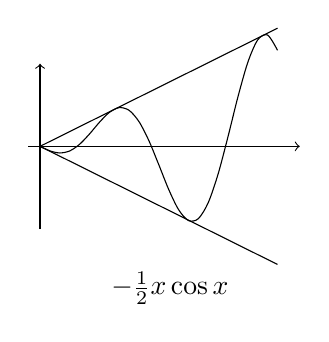
\begin{tikzpicture}[scale=0.3]
\draw[->](-0.5,0)--(3.5*pi,0);
\draw[->](0,-3.5)--(0,3.5);
\draw [smooth,black,domain=0:3.2*pi] plot (\x, {-0.5*\x *cos(\x r)});
\draw(0,0)--(3.2*pi,5);
\draw(0,0)--(3.2*pi,-5);
\node[] at (1.75*pi,-6) {$-\frac{1}{2}x\cos x$};
\end{tikzpicture}
\end{center}

\end{minipage}
\end{figure}
\end{enumerate}
\subsection*{Zusatzbedingungen einer DGL. Anfangs und Randbedingungen}
Die in der allgemeinen Lösung einer DGL $n-$ter Ordnung auftretenden Parameter lassen sich durch Zusatzbedingungen festlegen. Physikalisch sinnvolle Zusatzbedingungen werden meist in der Form von Anfangsbedingungen oder Randbedingungen vorgegeben. \\

Durch Vorgabe von derartigen Bedingungen eliminiert man die Parameter aus der allgemeinen Lösung der DGL und erhält damit eine partikuläre Lösung.
\subsubsection*{Beispiel 7.10}
Freier Fall mit Reibung
\begin{center}
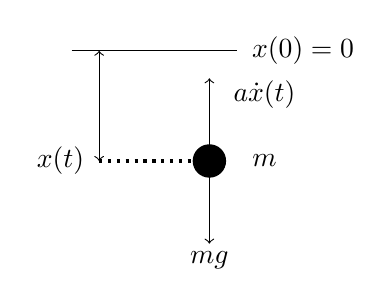
\begin{tikzpicture}[scale=0.7]
\node[circle,fill=black,inner sep=1.5mm] (a) at (0,0) {};
\draw[<->](-2,0)--(-2,2);
\draw[->] (0,0) -- (0,1.5);
\draw[->] (0,0) -- (0,-1.5);
\draw[] (-2.5,2) -- (0.5,2);
\draw[dotted, very thick] (-2,0) -- (0,0);
\node[] at (-2.7,0){$x(t)$};
\node[] at (1.7,2){$x(0)=0$};
\node[] at (1,0){$m$};
\node[] at (1,1.2){$a\dot x(t)$};
\node[] at (0,-1.8){$mg$};
\end{tikzpicture}
\end{center}
$m\ddot{x}=mg-a\dot{x}$. Anfangsbedingungen: $x(0)=0; v(0)=\dot{x}(0)=0$
\[mx''(t)+ax'(t)=mg\]
\[(H)\hspace{10mm}mx''(t)+ax'(t)=0\]
\[p(\lambda)=m\lambda^2+a\lambda=0\Rightarrow \lambda=0,\lambda=-\frac{a}{m}\]
\[x_h(t)=c_1+c_2e^{-\frac{a}{m}t}\]
Für die spezielle Lösung, wählen wir als Ansatz $x_s(t)=kt$
\[\left( \begin{array}{l}
b(t) = mg = {\text{ konstant, aber  }}{e^{0 \cdot t}} = 1 = {\text{ konstant}}\\
{\text{ist eine Lösung der }}(H)
\end{array} \right)\]
\[x'(t)=k\hspace{10mm}x''(t)=0\]
\[mx''(t)+ax'(t)=ak=mg\Rightarrow k=\frac{mg}{a}\]
Allgemeine Lösung
\[x(t)=x_h(t)+x_s(t)=c_1+c_2e^{-\frac{a}{m}t}+\frac{mg}{a}t\]
Anfangsbedingungen
\[x(0)=0=c_1+c_2=0\]
\[x'(t)=c_2\left(-\frac{a}{m}\right)e^{-\frac{a}{m}t}+\frac{mg}{a}=0\]
\[x'(0)=0\Rightarrow c_2\left( -\frac{a}{m}\right) +\frac{mg}{a}=0\]
\[c_2=\frac{m^2g}{a^2}\hspace{10mm}c_1=-\frac{m^2g}{a^2}\]
\[\Rightarrow x(t)=-\frac{m^2g}{a^2}+\frac{m^2g}{a^2}e^{-\frac{a}{m}t}+\frac{mg}{a}t\]
\[x(t)=\frac{mg}{a}t-\frac{m^2g}{a^2}\left[ 1-e^{-\frac{a}{m}t}\right]\]
Eine partikuläre Lösung einer DGL $n-$ter Ordnung \[y^{(n)}{(x)}+a_{n-1}(x)+\dots+a_0 y(x)=b(x)\] kann man aus der allgemeinen Lösung
\[y(x)=y(x,c_1,c_2,\dots,c_n)\] der DGL erhalten
\begin{itemize}
\item Durch die Vorgabe von Anfangsbedingungen
\[y(x_0)=A_0\]
\[y'(x_0)=A_1\]
\[y^{(n-1)}(x_0)=A_n\]
Funktionswert und weitere Ableitungen bis zur $(n-1)-$ten an einer speziellen Stelle $x_0$.
\item Durch die Vorgabe von Randbedingungen
\[y(x_1)=B_1, y(x_2)=B_2, \dots, y(x_n)=B_n\] Funktionswerte an $n$ verschiedenen Stellen
\end{itemize}
\subsubsection*{Beispiel 7.11}
Lineares Federpendel:
\[mx''(t)+K_1x=0, \omega^2=\frac{K}{m}\]
\[x''(t)+\omega^2x=0\hspace{10mm}(H)\]
\[p(\lambda):\lambda^2+\omega^2=0\Rightarrow\lambda_{1,2}=\pm\omega i\]
Homogene Lösung: $x_h(t)=c_1\cos\omega t+c_2\sin\omega t$.
Wenn wir die folgenden Zusatzbedingungen haben
\begin{enumerate}[(i)]
\item $x(0)=1, x'(0)=2\omega$
\[x'(t)=-c_1\omega\sin\omega t+c_2\omega\cos\omega t\]
\[x(0)=1\Rightarrow c_1\cos 0+c_2\sin 0=c_1=1\]
\[x'(0)=2\omega\Rightarrow-c_1\omega\sin 0+c_2\omega\cos 0=2\omega\]
\[\Rightarrow \omega c_2=2\omega\Rightarrow c_2=2\]
\[\Rightarrow x_p(t)=\cos\omega t+2\sin\omega t\]
\item Mit Randbedingungen: $x(0)=1$, $x\left(\frac{\pi}{2\omega}\right)=1$
\[x(0)=c_1\cos 0+c_2\sin 0=c_1=1\]
\[x\left(\frac{\pi}{2\omega}\right)=c_1\cos\frac{\pi}{2}+c_2\sin\frac{\pi}{2}=c_2=1\]
Also $x_p(t)=\cos\omega t+\sin\omega t$
\end{enumerate}

\section{Lineare DGL erster Ordnung (mit allgemeinen Koeffizienten)}
Die LDGL hat die allgemeine Form (mit $b(x)$ als inhomogener Term) \[y'(x)=a(x)y+b(x)\]
\noindent Und $y'(x)=a(x)y$ ist die zugehörige homogene Gleichung. \\

\noindent Lösung von $y'(x)=a(x)y$: \[\frac{y'(x)}{y(x)}=a(x)\]
d.h. $\left( \ln y(x)\right)'=a(x)$. Sei $A(x)$ eine Stammfunktion von $a(x)$, so ist \[\ln y(x)=A(x)+c\] Also $y(x)=e^{A(x)}\cdot e^c=Ke^{A(x)}$
\subsubsection*{Satz 7.12}
Die allgemeine Lösung von $y'=ay$ ist $y(x)=Ke^{A(x)}$ wobei $K\in\R$ und $A'(x)=a(x)$
\subsubsection*{Beispiel}
\[xy'-2y=0\]
\[y'=\frac{2}{x}y\Rightarrow a(x)=\frac{2}{x}, A(x)=2\ln\abs{x}=\ln x^2\]
\[e^{A(x)}=e^{\ln x^2}=x^2\]
\[\Rightarrow\text{ Lösung von }y'(x)=\frac{2}{x}y \Rightarrow y(x)=Kx^2\]
Jetzt suchen wir eine spezielle Lösung von $y'=a(x)y+b(x)$
\subsubsection*{Ansatz}
$y=uv$ wobei $u,v$ Funktionen sind. Dann ist \[y'=u'v+uv'\] und \[a(x)y+b(x)=ay+b=u'v+uv'\]
\[a(uv)+b=u'v+uv'\]
\[\Rightarrow u'v+u\lbrack v'-av\rbrack =b\]
Jetzt wählen wir $v$, so dass \[v'-av=0\]d.h. \[v=e^{A(x)}\] Dann ist $u'v=b$ d.h. $u'=be^{-A(x)}$ d.h. $u$ ist eine Stammfunktion von $be^{-A(x)}$

\subsubsection*{Satz 7.13}
Seien $A(x)$ eine Stammfunktion von $a(x)$ und $U(x)$ ein Stammfunktion von $be^{-A(x)}$. Dann ist $y(x)=e^{A(x)}* U$ Lösung von $y'=a(x)y+b(x)$

\subsubsection*{Korollar 7.14}
Die Allgemeine Lösung der LDGL $y'=ay+b$ ist durch $y(x)=e^{A(x)}\int{b(x)e^{-A(x)} dx}+Ke^{A(x)}$ gegeben, wobei $K\in\R$, $A(x)$ eine Stammfunktion von $a(x)$ ist.

\subsubsection*{Beispiel 7.15}
\begin{enumerate}
\item \[xy'-2y=2x^4\]
\[\Rightarrow y' = \underbrace {\frac{2}{x}}_{a(x)}y + \underbrace {2{x^3}}_{b(x)}\]
\[A(x)=2\ln\abs{ x }=\ln x^2\]
\[Ke^{A(x)}=Kx^2\text{ ist die Lösung der homogenen DGL }y'=ay\]
Wir bestimmen jetzt die Stammfunktion von \[b(x)\cdot e^{-A(x)}=2x^3e^{-\ln (x)^2}=2x^3 x^{-2}=2x\]
\[2\frac{x^3}{x^2}=2x\]
Also $b(x)e^{-Ax}$ ist eine Stammfunktion von $\int{2xdx=x^2}$ und $x^2e^{A(x)}=x^4$. Somit ist die allgemeine Lösung \[y(x)=x^4+Kx^2\]
\item \[y'=4x+5y-3\]
\[y' - \underbrace 5_ay = \underbrace {4x - 3}_b\]
LDGL mit konstanten Koeffizienten. Störfunktion ist  $4x-3$.\\

\noindent HDGL: \[y'-5y=0\]
\[\frac{y'}{y}=5\]
\[\ln y(x)=5x+c\]
\[y_h(x)=Ke^{5x} \text{ Hom. Lösung}\]
\[A(x)=5x\]
Spez. Lösung: Sei $U(x)$ Stammfunktion von $(4x-3)e^{-5x}$. Dann ist die spezielle Lösung \[e^{5x}U(x)=e^{5x}\int{(4x-3)e^{-5x}dx}\]
\[ \int {\underbrace {(4x - 3)}_u\underbrace {{e^{ - 5x}}}_{v'}dx} \]
\[\mathop = \limits^{P.I.} (4x - 3)\frac{{{e^{ - 5x}}}}{{ - 5}} + \frac{4}{5}\int {{e^{ - 5x}}dx}\]
\[ = \left[ {\left( {\frac{{4x - 3}}{{ - 5}}} \right) - \frac{4}{{25}}} \right]{e^{ - 5x}}\]
\[ = \left( {\frac{{ - 4x}}{{ - 5}} + \frac{{11}}{{25}}} \right){e^{ - 5x}}\]
\[\Rightarrow \text{ Spezielle Lösung: }y_s(x)=e^{5x}\cdot U(x)=\frac{-4x}{5}+\frac{11}{25}\]
Allgemeine Lösung: \[y(x)=Ke^{5x}-\frac{4x}{5}+\frac{11}{25}\]
\end{enumerate}

\section{Separierbare DGL}
\begin{definition}{7.16}
Eine separierbare DGL ist von der Form \[y'=f(x)g(y)\]
\end{definition}
Ein einfaches Verfahren, die so genannte ``Separation der Variablen'', lässt sich anwenden, wenn die DGL separierbar ist. Der ``Trick'': Wir trennen die Terme voneinander und integrieren dann. Dabei ist es hilfreich, $y'=\frac{dy}{dx}$ zu schreiben und die Formel $dy$ bzw. $dx$ als Zähler bzw. Nenner des Bruches aufzufassen.

\subsubsection*{Beispiel 7.17}
\begin{enumerate}
\item \[y'=2xy\]\[\begin{array}{l}
\begin{array}{*{20}{c}}
{\frac{{dy}}{{dx}} = 2xy}\\
{}
\end{array}\begin{array}{*{20}{c}}
 \Rightarrow \\
 \downarrow
\end{array}\begin{array}{*{20}{c}}
{\frac{{dy}}{y} = 2xdx}\\
{}
\end{array}\\
{\text{trennen formel }}x{\text{ bzw }}y{\text{ - Terme}}
\end{array}\]
Jetzt integrieren wir auf beiden Seiten \[\int{\frac{dy}{y}}=\int{2xdx}\]
\[\ln\abs{ y}=x^2+c\]Da wir an der Lösung $y$ interessiert sind und nicht am Logarithmus davon, wenden wir die Exponentialfunktion an \[\abs{ y}=e^{x^2+c}=e^ce^{x^2}\]
Links und rechts stehen nur positive Grössen. Wenn wir aber auf der rechten Seite nicht nur positive konstante $e^c>0$ zulassen, sondern irgendwelche Konstanten $K\in\R$ erhalten wir \[y(x)=Ke^{x^2}\]
\item \[y'=1+y^2\text{ ist separierbar}\]
\[\int{\frac{dy}{1+y^2}=\int{dx}}\]
\[\Rightarrow \arctan y=x+c \Leftrightarrow y=\tan(x+c)\]
\end{enumerate}
\subsubsection*{Bemerkung 7.18}
$y'=f(x)g(x)$ hat die konstanten Lösungen $y=y_0$ für alle $y_0$ mit $g(y_0)=0$. Der Fall $g(y)=0$ muss gesondert betrachtet werden.
\begin{enumerate}
\item[3.] \[\abs{ x}, \abs{ y}<1,y'=\sqrt{\frac{1-y^2}{1-x^2}}\]
hat keine konstanten Lösungen
\[\frac{{dy}}{{\sqrt {1 - {y^2}} }} = \frac{{dx}}{{\sqrt {1 - {x^2}} }} \Rightarrow \int {\frac{{dy}}{{\sqrt {1 - {y^2}} }}}  = \int {\frac{{dx}}{{\sqrt {1 - {x^2}} }}} \]
\[\Rightarrow \arcsin y=\arcsin x+c\]
\[y=\sin\lbrack\arcsin x+c \rbrack\]
\[=x\cos c\pm\sqrt{1-x^2}\sin c\]
\[=ax+b\sqrt{1-x^2}\]
wobei $a,b\in\R$ mit $a^2+b^2=1$. Rückeinsetzen in die DGL liefert die Zusatzbedingung \[y'=a-\frac{bx}{\sqrt{1-x^2}}>0,\hspace{5mm} (1+y^2>0)\]
\end{enumerate}
